\section{IPFS}
\begin{frame}
	\frametitle{IPFS}
	\vspace{-\baselineskip}
	\begin{center}
		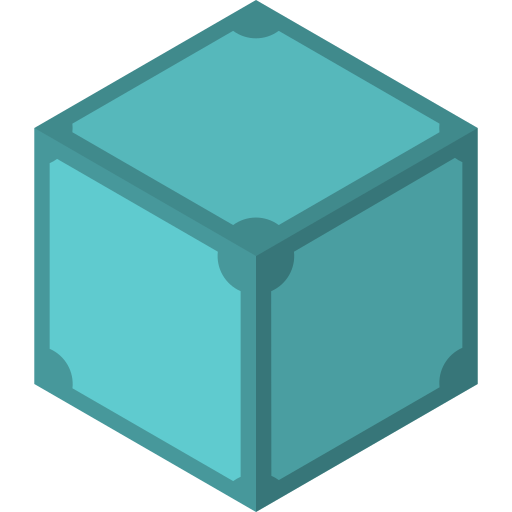
\includegraphics[width=.1\paperwidth]{assets/figures/ipfs-logo}
	\end{center}
	IPFS - κατανεμημένο σύστημα αποθήκευσης
	\begin{itemize}
		\item Δίκτυο ομότιμων κόμβων (P2P)
		\item Διευθυνσιοδότηση περιεχομένου (content addressing)
		\item Καρφίτσωμα δεδομένων (pinning)
	\end{itemize}
\end{frame}

\note{
	Συνεχίζουμε με το τρίτο επίπεδο της στοίβας. Όπως είπαμε, για την αποθήκευση του κύριου όγκου των δεδομένων επιλέχθηκε το IPFS. Αυτό έγινε γιατί η αποθήκευση δεδομένων επί του blockchain μεταφράζεται πάντα σε επιπλέον κόστη συναλλαγών, τα οποία στην περίπτωσή μας θα ήταν απαγορευτικά μεγάλα. 
	
	Με ΠΟΛΥ απλοϊκό τρόπο το IPFS μπορεί να παρομοιασθεί με τα torrents. Πρόκειται δηλαδή για ένα κατανεμημένο σύστημα ομότιμων κόμβων, το οποίο αποθηκεύει και παρέχει  δεδομένα.
	
	Εδώ το περιεχόμενο δεν προσδιορίζεται από την τοποθεσία (π.χ. HTTP), άλλα από το τι περιλαμβάνει. Έχουμε δηλαδή διευθυνσιοδότηση του περιεχομένου (content addressing), κάθε κομμάτι του οποίου αποκτά ένα μοναδικό αναγνωριστικό.
	
	Τέλος θα πρέπει να σημειώσουμε πως οι κόμβοι που διαθέτουν και διαμοιράζουν το περιεχομενο αντιμετωπίζουν, ως προεπιλογη, τα αποθηκευμένα δεδομένα ως προσωρινή μνήμη. Για την αποφυγή της διαγραφής των δεδομένων τα δεδομένα θα πρέπει να καρφιτσωθούν δηλαδή να γίνουν pinned από τους κόμβους. 
}